\documentclass[10 pt,usenames,dvipsnames, oneside]{article}
\usepackage{../../../modelo-ensino-medio}



\begin{document}

\begin{center}
  \begin{minipage}[l]{3cm}
\includegraphics[width=2cm]{logo}    
\end{minipage}\hfill
\begin{minipage}[r]{.8\textwidth}
 {\Large \scshape Atividade: Estádio de Futebol}  
\end{minipage}
\end{center}
\vspace{.2cm}

\ifdefined\prof
%Habilidades da BNCC
% \begin{objetivos}
% \item 
% \end{objetivos}

%Caixa do Para o Professor
\begin{goals}
%Objetivos específicos
\begin{enumerate}
\item Apresentar a possibilidade de outros tipos de equações.
\item Familiarizar o aluno com a ideia de que curvas no plano podem ser representadas algebricamente por equações, e vice-versa.
\item Usar o Geogebra para resgatar a ideia de sistemas de equações
\end{enumerate}

\tcblower

%Orientações e sugestões
\begin{itemize}
\item Nessa atividade, vamos acrescentar mais um conjunto solução de uma classe bem específica de equações: a equação de uma elipse mas é apenas a título de exemplo
\item O objetivo é que o aluno se familiarize com a ideia de que curvas no plano podem ser representadas algebricamente por equações, e vice-versa - mas não nos aprofundaremos muito em modelos de equação que não sejam as equações polinomiais do primeiro e segundo graus.
\item Problematize junto aos alunos o motivo do centro do campo estar associado à origem do sistema cartesiano. Auxilie-os a perceber que a curva a que nos referimos - no caso, o contorno do Mineirão - seria a mesma em qualquer posição dentro do sistema de eixos cartesianos, com os eixos contendo seus pontos máximos  ou não, mas que essas configurações não são interessantes porque as equações assim geradas seriam bem mais complexas.
Essa situação pode ser experimentada da seguinte maneira: Abra uma tela do GeoGebra, cole a imagem do Mineirão e rotacione. Tome 5 pontos no contorno mais externo da imagem do estádio e gere a cônica que passa por esses 5 pontos. Por exemplo:
{\footnotesize https://www.geogebra.org/classic/ujwf9gdx}  
\item Nos itens \titem{a)} e \titem{b)}, o professor deve ajudar o aluno a perceber que os pontos dos eixos $x$ e $y$ obedecem às equações $y=0$  e $x=0$, respectivamente.
\item No item \titem{c)}, a proposta é que o aluno busque livremente esses valores, da mesma forma que realizado com o \hyperref[castelo]{\textit{Enigma do Castelo}}.
\end{itemize}
\end{goals}

\bigskip
\begin{center}
{\large \scshape Atividade}
\end{center}
\fi

O Estádio Governador Magalhães Pinto, mais conhecido como Mineirão, é um estádio de futebol localizado em Belo Horizonte, capital de Minas Gerais. Na \fref{mineirao}, pode-se ver uma foto da vista aérea do estádio através do \emph{Google Earth}. O contorno externo do estádio, realçado na figura por uma linha azul, é aproximado por uma elipse. Suponha que tenham sido introduzidas coordenadas cartesianas e unidades de medida de comprimento nesta foto. A origem $O$ foi escolhida para ser o centro do campo de futebol e os pontos $(x, y)$ do contorno externo do estádio são exatamente aqueles que são soluções da equação $9x^2 = 144 - 16y^2$.



\begin{figure}[H]
\centering

\noindent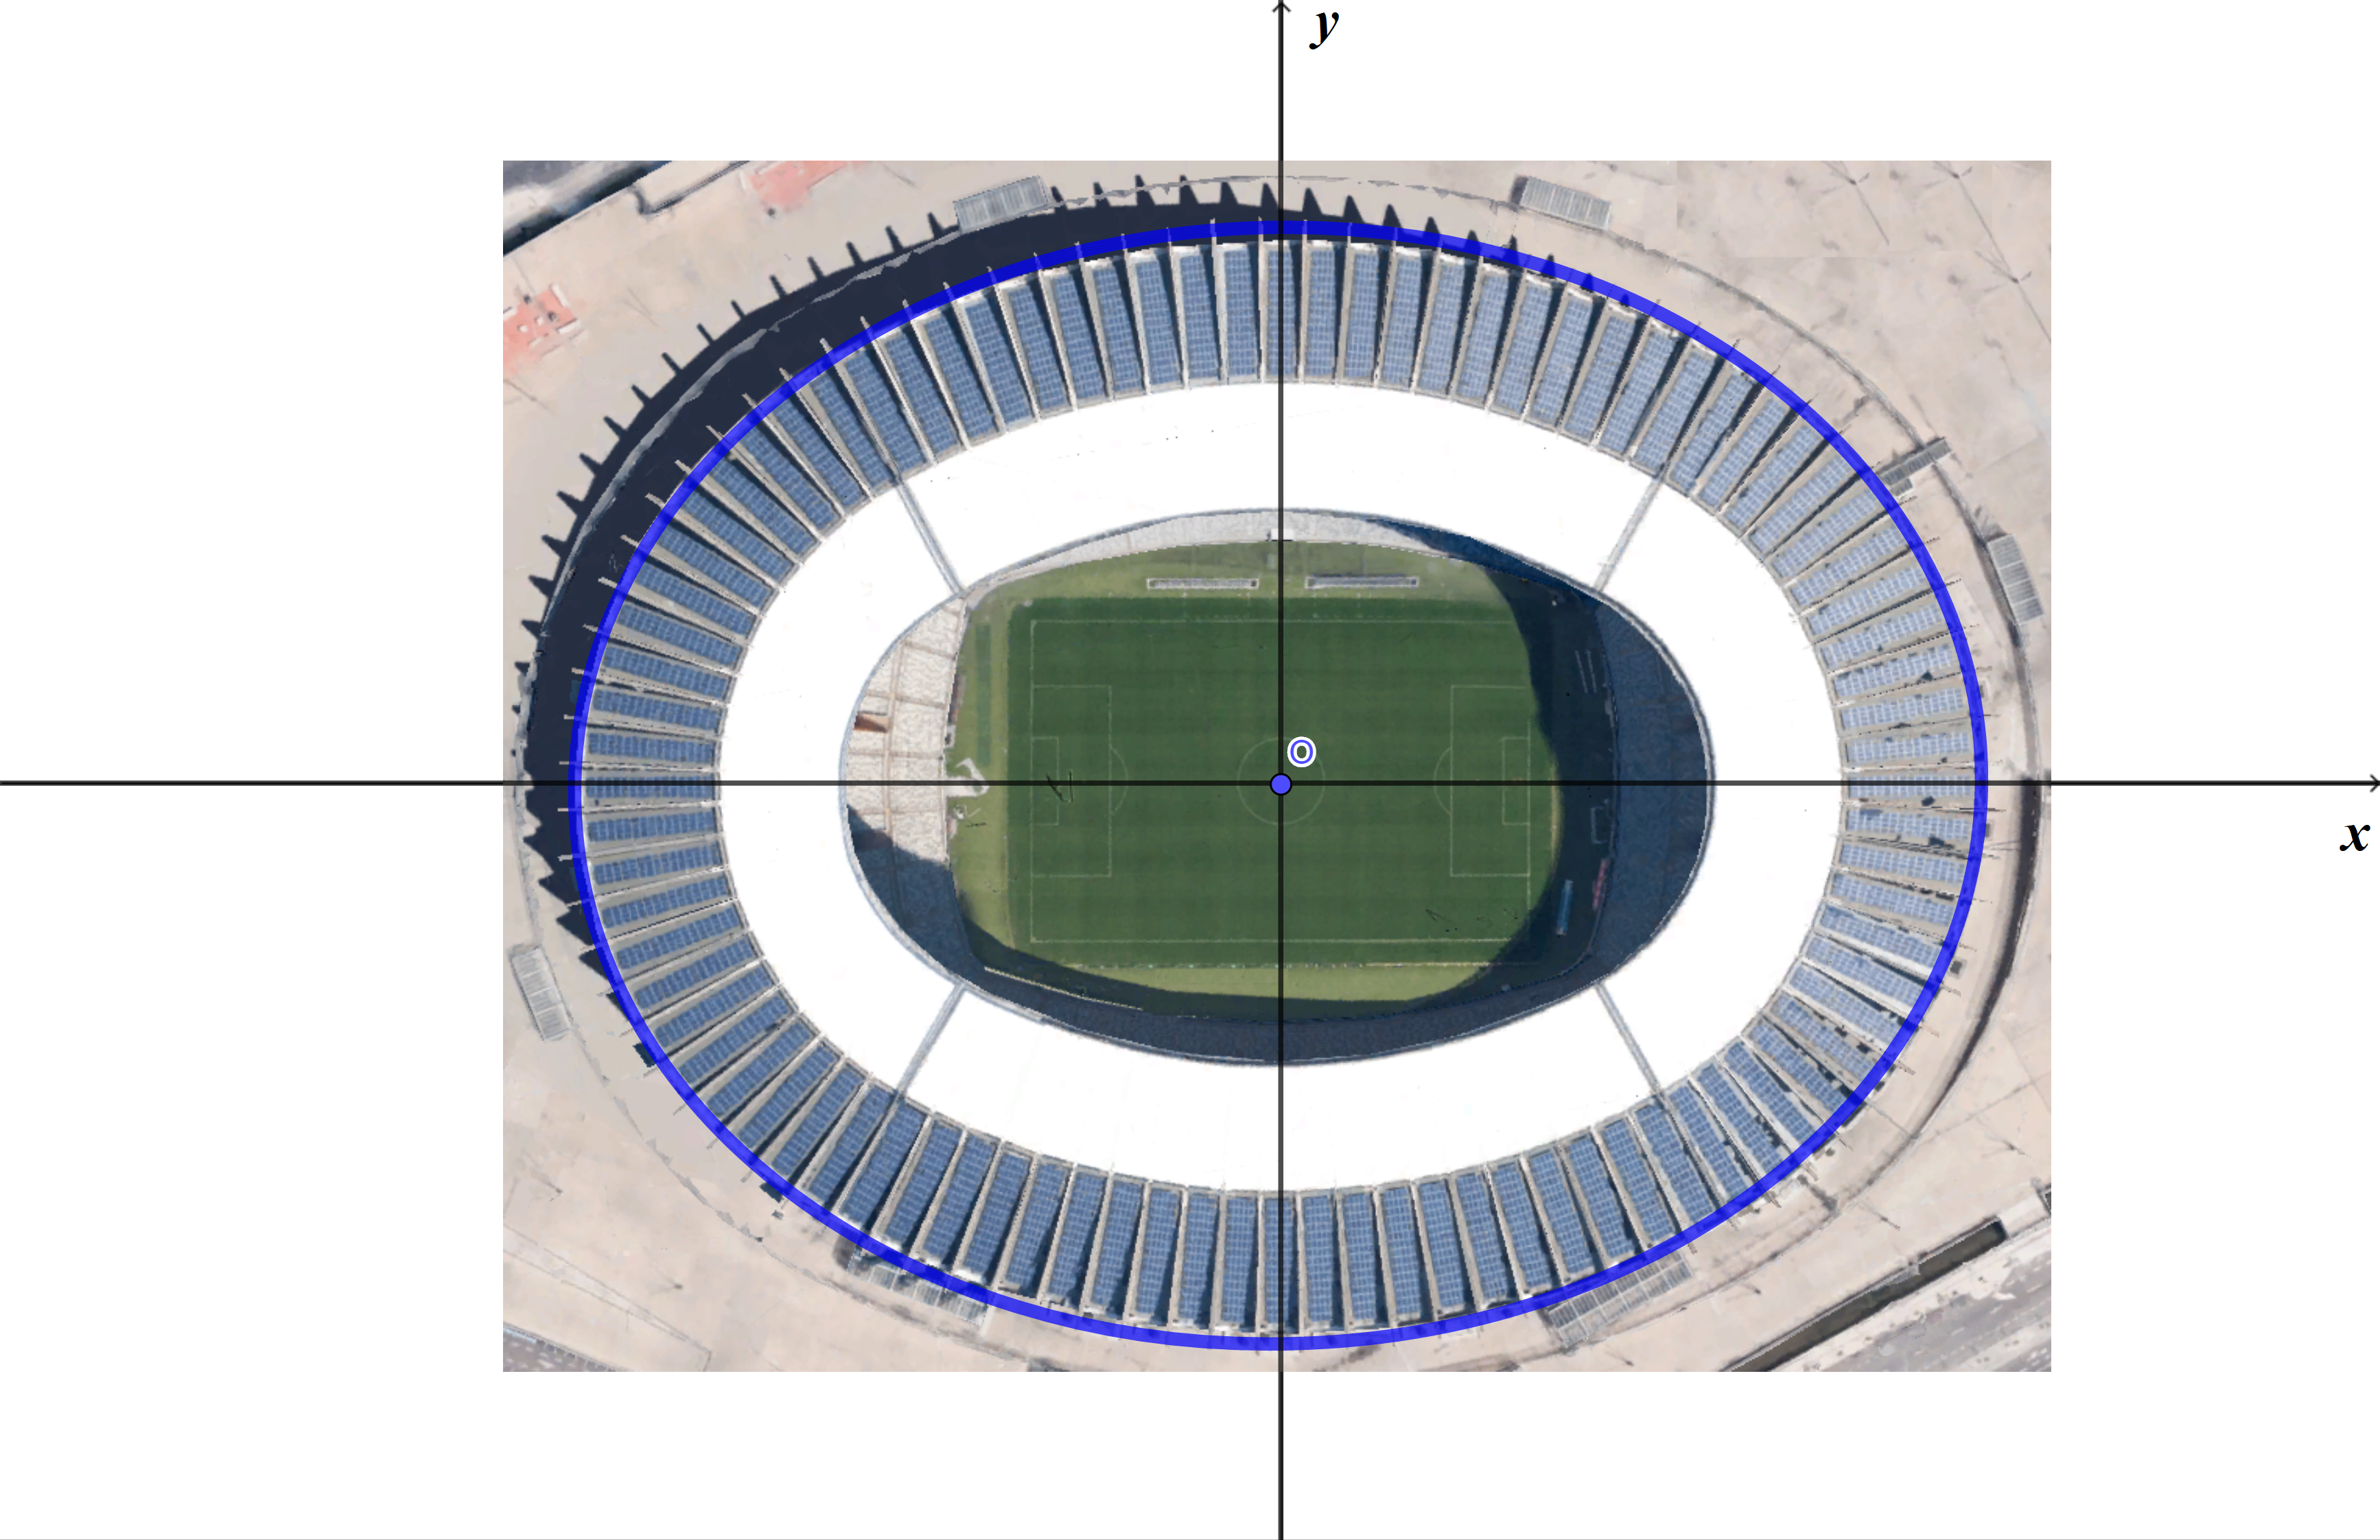
\includegraphics[width=300bp]{mineirao_com_eixos.png}
\caption{Estádio do Mineirão com os eixos marcados}
\label{mineirao}
\end{figure}

\begin{enumerate}

\item{} 
Qual a distância entre os pontos do contorno externo do Mineirão que estão sobre o eixo $x$?

\item{}
Qual a distância do centro do campo de futebol a qualquer um dos dois pontos do contorno externo do estádio que estão sobre o eixo $y$?

\item{}
Existe algum ponto $(a,b)$ do contorno externo do Mineirão que não esteja sobre os eixos coordenados de modo que $a$ e $b$ sejam números inteiros? Justifique.


\end{enumerate}

\ifdefined\prof
\begin{solucao}

\begin{enumerate}
\item $8.$
\item $3.$
\item Não. Faça os alunos perceberem que os valores de $x$ variam entre $-4$ e $4$, que os valores de $y$ variam entre $-3$ e $3$ e testarem os candidatos vendo que não satisfazem a equação.
\end{enumerate}

\end{solucao}
\fi

\end{document}